\chapter{Технологическая часть}

\section{Выбор языка программирования и среды разработки.}

Для решения описанной задачи был выбран язык программирования C\# \cite{Microsoft}.
Данный язык был выбран по следующим причинам.

\begin{enumerate}
	\item Он использует объектно-ориентированный подход к программированию.
	\item В языке присутствует обилие синтаксических возможностей,
	      которые помогают использовать готовые конструкции,
	      вместо того, чтобы переписывать однотипные строки кода.
	\item В нём имеется большое количество библиотек и шаблонов,
	      позволяющих не тратить время на изобретение готовых конструкций.
	\item Язык является строго типизированным,
	      что позволяет защититься от непроконтролированных ошибок.
	\item Он является нативным, что необходимо
	      для уменьшения времени работы алгоритмов с помощью распараллеливания.
\end{enumerate}

В качестве среды разработки был использован Visual Studio Code \cite{Vs}.
Visual Studio Code подходит не только для  Windows \cite{Win},
но и для Linux \cite{Lin}, это причина,
по которой был выбран VS code,
т.к. на моем компьютере установлена ОС Ubuntu 18.04.4 \cite{Ubuntu}.
Также моей архитектуре присутствует 8 ядер.
Для замеров времени использовался класс Stopwatch \cite{Stopwatch}.

% \section{Сведения о модулях программы}
\section{Структура программы}

Данная программа состоит из следующих модулей.

\begin{itemize}
	\item Program.cs - файл, содержащий точку входа в программу.
	\item Vector.cs - файл, содержащий класс Vector, в котором
	      написаны основные методы для работы с вектором.
	\item Color.cs - файл, содержащий класс Color, в котором
	      написаны основные методы для работы с цветом.
	\item Constants.cs - файл, содержащий константы.
	\item Shape.cs - файл, содержащий базовый класс Shape
	      и унаследованные от него классы Sphere и Cylinder.
	\item Light.cs - файл, содержащий класс Light.
	\item MinForm.cs - файл, содержащий интерфейс и алгоритм трассировки лучей.
\end{itemize}

На рисунках \ref{fig:class_diagram1} - \ref{fig:class_diagram2} показана структура классов.

\begin{figure}[ht!]
	\centering{
		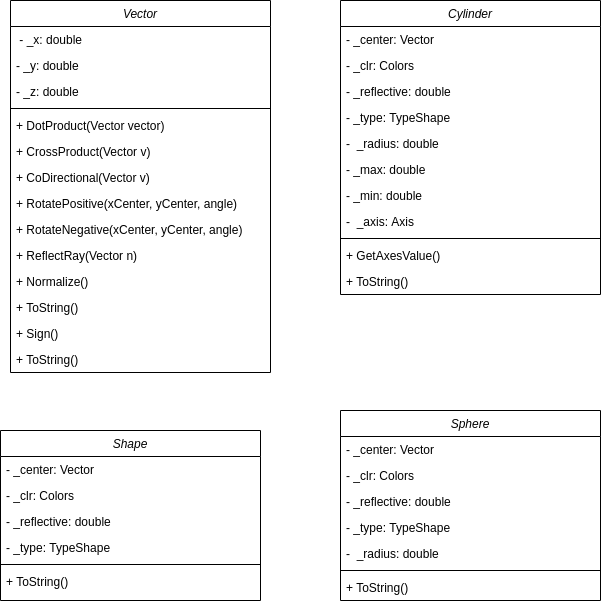
\includegraphics[width=0.7\textwidth]{class_diagram1.png}
		\caption{Структура классов (начало)}
		\label{fig:class_diagram1}}
\end{figure}

\begin{figure}[ht!]
	\centering{
		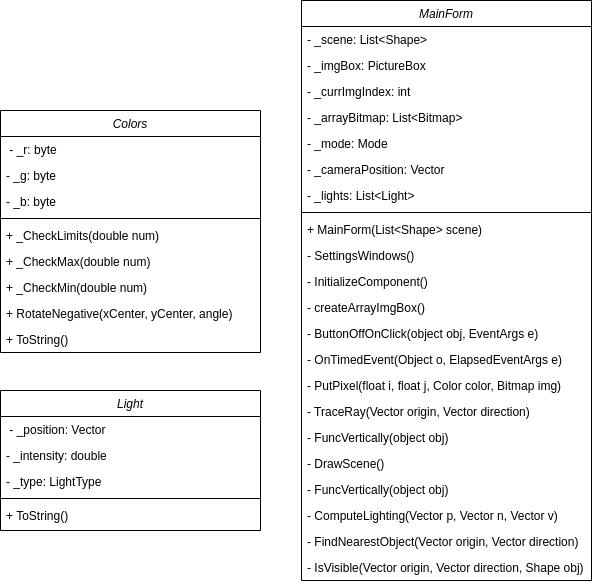
\includegraphics[width=0.7\textwidth]{class_diagram2.png}
		\caption{Структура классов (окончание)}
		\label{fig:class_diagram2}}
\end{figure}

\newpage
На листинге 3.1 представлен основной код алгоритма.

\newpage
\begin{lstlisting}[label=some-code,caption=Трассировка лучей.]
private Colors TraceRay(Vector origin, Vector direction, double min_t, double max_t, int depth = 3)
{
	double closest_t = Double.PositiveInfinity;
	Shape ClosestObject = FindNearestObject(origin, direction, min_t, max_t, ref closest_t);
	if (ClosestObject == null)
		return new Colors(0, 0, 0);

	Vector point = origin + direction * closest_t;
	Vector tmp = null;
	if (ClosestObject.Type == TypeShape.Sphere)
	{
		tmp = ClosestObject.Center;
	}
	else if (ClosestObject.Type == TypeShape.Cylinder)
	{
		Cylinder cylinder = ClosestObject as Cylinder;

		Vector axesValue = cylinder.GetAxesValue();   
		Vector axesValueRev = cylinder.GetAxesValue(); 		
		axesValueRev.Reverse();

		axesValue = axesValue * cylinder.Center; 
		axesValueRev = axesValueRev * point;
		tmp = axesValue + axesValueRev; 
	}

	Vector normal = point - tmp;
	normal = normal * (1.0d / normal.Length);
	Vector view = direction * -1.0d;
	double lighting = ComputeLighting(point, normal, view);

	Colors result = ClosestObject.Clr * lighting;

	if (depth <= 0)
		return result;

	Vector reflected_ray = ReflectRay(view, normal);
	Colors reflected_color = TraceRay(point, reflected_ray, 0.001d, Double.PositiveInfinity, depth - 1);

	double reflective = ClosestObject.Reflective;
	return result * (1 - reflective) + reflected_color * reflective;
}
\end{lstlisting}

\section{Интерфейс и тестирование}

На рис. \ref{fig:interface} показан интерфейс программы.
По нажатию на кнопку механическая система начинает движение.
Повторное нажатие приводит к останову/запуску системы, в зависимости от
состояния в котором она находилась до нажатия.

\begin{figure}[ht!]
	\centering{
		
\includegraphics[width=0.7\textwidth]{interface.png}
		\caption{Интерфейс}
		\label{fig:interface}}
\end{figure}

Тестирование проводится по методу черного ящика.
На вход программы подается файл, содержащий сцену (таблица \ref{table:ref1}).
Результатом является изображение рис. \ref{ref:res1}, показывающее корректность работы программы.

\begin{table}
	\centering
	\begin{tabular}{| l |}
		\hline
		1  -1.6 0.2 7 0.8 192 192 192 0.2     \\ \hline
		1 0 0.2 7 0.8 192 192 192 0.2         \\  \hline
		1 1.6 0.2 7 0.8 192 192 192 0.2       \\  \hline
		2 -3 0 5 0.15 255 255 255 0 -1.1 2 1  \\  \hline
		2 3 0 5 0.15 255 255 255 0 -1.1 2 1   \\  \hline
		2 -2 2 5 0.15 255 255 255 0 -1 5 0    \\  \hline
		1 -3 2 4.97 0.2 255 255 255 0         \\  \hline
		1 3 2 4.97 0.2 255 255 255 0          \\  \hline
		2 -3 0 10 0.15 255 255 255 0 -1.1 2 1 \\  \hline
		2 3 0 10 0.15 255 255 255 0 -1.1 2 1  \\  \hline
		2 -2 2 10 0.15 255 255 255 0 -1 5 0   \\  \hline
		1 -3 2 10 0.2 255 255 255 0           \\  \hline
		1 3 2 10 0.2 255 255 255 0            \\  \hline
	\end{tabular}
	\caption{Входные данные}
	\label{table:ref1}
\end{table}


\section{Вывод}

В данном разделе был выбран ЯП и среда разработки.
Также описаны модули и разобран листинг рис 3.1, показывающий работу алгоритма.